\chapter{Lattice based algorithms}
\label{ch:block_diagrams}

\begin{figure}[ht!]
  \centering
  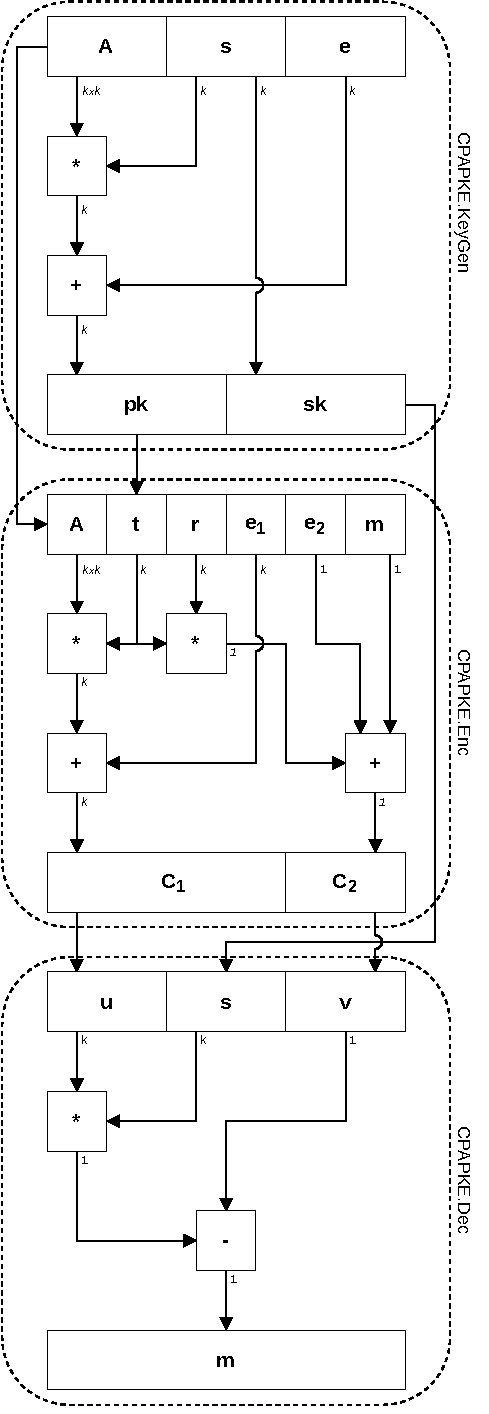
\includegraphics[width=0.484\textwidth]{pictures/kyber_all.pdf}
  \caption{Kyber block scheme}
  \label{img:kyber_all}
\end{figure}

\begin{figure}[ht!]
  \centering
  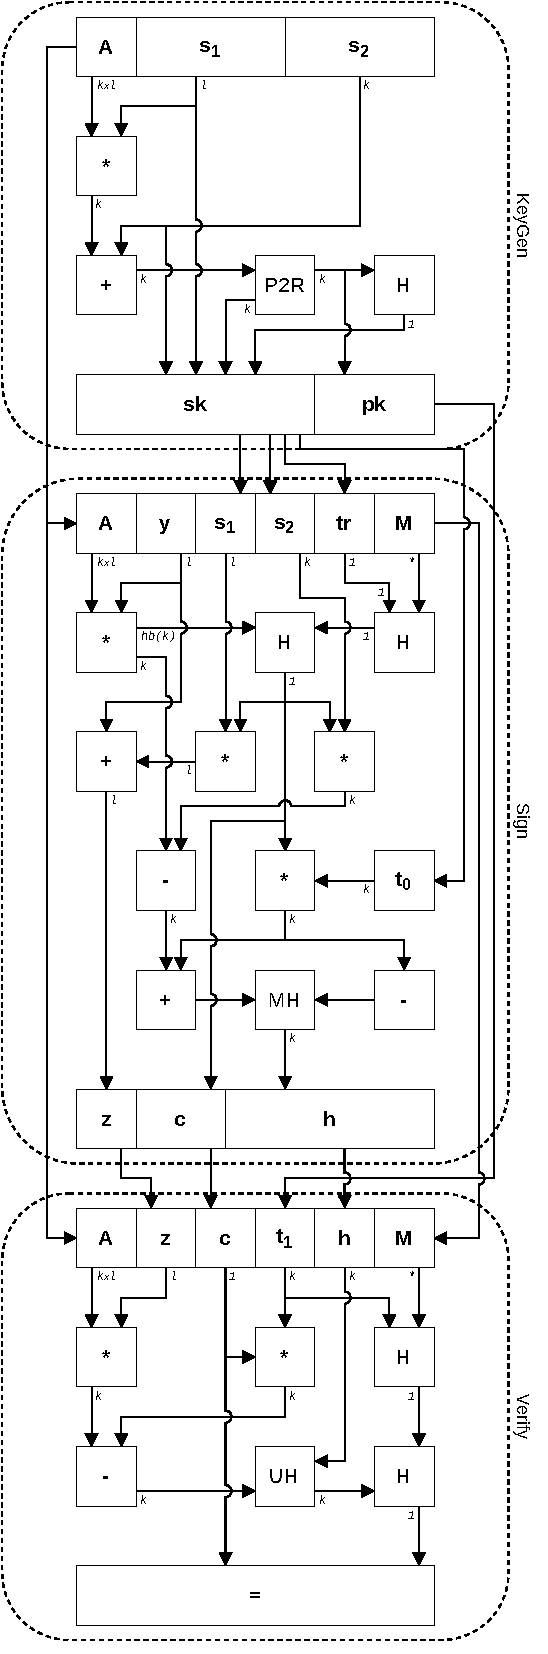
\includegraphics[width=0.497\textwidth]{pictures/dil_all.pdf}
  \caption{Dilithium block scheme}
  \label{img:dil_all}
\end{figure}

\chapter{Go program instructions}
This appendix contains the necessary information for building the go program, running it and then instructions on how to run the provided tests.
\label{ch:go_instructions}
\section{How to build}
Go supports most of the well know operating systems such as Linux, Windows and Mac. First of all download the latest version of the go binary from this link
\begin{itemize}
  \item \url{https://go.dev/doc/install}.
\end{itemize}
Once go is installed the binary for this thesis can be built by running
\begin{itemize}
  \item \texttt{go build -v}
\end{itemize}
inside the command line interface of your operating system. The command also has to be ran inside the root directory of the project. The output of this command should yield a~file named \texttt{main.exe} for Windows or \texttt{main} for other operating systems.
\section{How to run}
Once the binary is built it can be ran just like any other binary. For Linux run with
\begin{itemize}
  \item \texttt{./main}
\end{itemize}
and for Windows run with
\begin{itemize}
  \item \texttt{main}
\end{itemize}
in your command line interface. Rest of the examples will be applicable to the Linux operating system. Additionally the option \texttt{-i} can also be specified to change the~number of iterations for the benchmark. For example to run benchmark with 5000 iterations run
\begin{itemize}
  \item \texttt{./main -i 5000}
\end{itemize}
The default value for number of iterations is 1000.
\section{How to test}
Tests that check whether the implementations are working correctly can be ran by entering
\begin{itemize}
  \item \texttt{go test -v}
\end{itemize}
into the command line interface in the root directory of the project.
